\chapter{Regelbasierte Wissensverarbeitung und Expertensysteme}

In vielen F�llen reichen typische numerische Herangehensweisen an Probleme nicht aus und es ist menschliche Expertise erforderlich. Dienstleistungen von Experten sind jedoch nicht immer verf�gbar und teuer. Mit der Anwendung symbolischer Probleml�sung unter Verwendung wissensbasierter Systeme (siehe Kapitel~\ref{chap:knowledge-based-systems}) kann menschliches Fachwissen mithilfe von Computern automatisiert und skaliert werden. Diese Systeme sind als Expertensysteme bekannt.

Einige Anwendungsbeispiele f�r Expertensysteme w�ren im Dienst der Medizin, wo viele seit rund 30 Jahren im Einsatz sind, in der Wirtschaft, wo es zur Kreditw�rdigkeitspr�fung und zum Abw�gen von Investitionsrisiken verwendet wird, und in Kundendienst-Chatbots.

\section{Aufbau eines regelbasierten Wissensbasierten Systems}

Regelbasierte Systeme basieren auf dem Prinzip eines Produktionssystems zur Termersetzung (Emil Post 1943). Eine �bersicht �ber ein komplettes Produktionssystems ist in Abbildung~\ref{fig:xps-overview} dargestellt.

\begin{figure}[H]
    \centering
    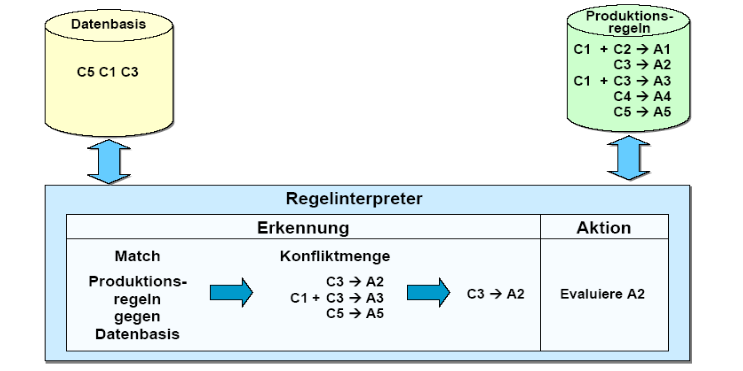
\includegraphics[width=0.9\textwidth]{figures/kap7/overview-xps.png}
    \caption{Produktionssystems zur Termersetzung}
    \label{fig:xps-overview}
\end{figure}

Eine Produktion, auch als ``Regel'' bekannt, besteht aus zwei Teilen (Abb.~\ref{fig:xps-regelstruktur}).

\begin{figure}[H]
    \centering
    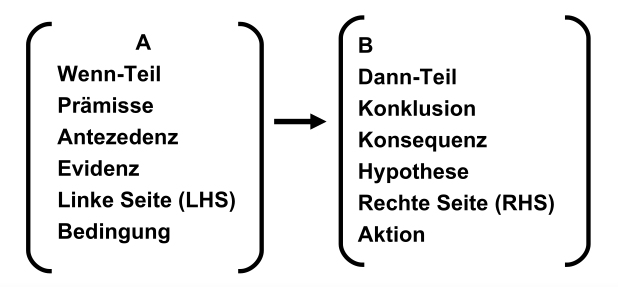
\includegraphics[width=0.8\textwidth]{figures/kap7/production-system-parts.png}
    \caption{Regelstruktur eines regelbasierten Expertensystems}
    \label{fig:xps-regelstruktur}
\end{figure}

Grunds�tzlich basieren die Regeln auf einer Kombination der Teile von A und Teilen von B. Zum Beispiel: Wenn A1 und A2 und An, \textbf{dann} B1 und B2 und Bn und Bm und so weiter. 

Anhand dieser Regeln kann Wissen von Experten gebildet werden. Tats�chlich arbeiten viele Expertensysteme mit einer einfachen Form von IF <Begingung> THEN <Konsequenz>.

\section{Zustandsraumdarstellung eines Wissensverarbeitungsproblems}

Die vier wichtigsten Komponenten f�r so ein System, die man kennen muss, sind Fakten, Regeln und Anfragen. 

\textbf{Fakten} sind Eintr�ge in der Fakten- oder Datenbasis. F�r jedes Problem beginnt das System mit einer Beschreibung des gesamten bekannten Wissens �ber eine Problemstellung. 

\textbf{Regeln} werden verwendet, um einen L�sungsschritt zu erzeugen. Mit Hilfe von Regeln werden neue Fakten ber�cksichtigt und einige fr�here verworfen. Das bedeutet, dass die Faktenbasis durch die Anwendung von Regeln ver�ndert wird.

\textbf{Anfragen}, die als Pr�dikate konstruiert sind, beschreiben die Bedingungen, die ein Problem umgeben. Wenn das Pr�dikat in der Datenbasis gefunden wird (nachdem Fakten einige Regeln durchlaufen haben), ist das Problem gel�st.  

Eine �bersicht �ber die Beziehungen zwischen diesen drei Komponenten ist in Abbildung~\ref{fig:xps-relationships} dargestellt.

\begin{figure}[H]
    \centering
    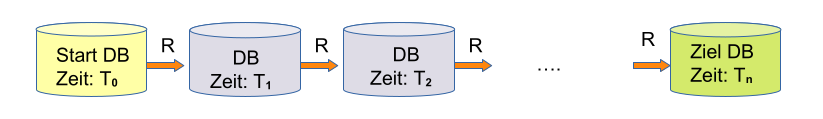
\includegraphics[width=\textwidth]{figures/kap7/state-space-of-xps.png}
    \caption{Beziehung zwischen Fakten, Regeln und Abfragen}
    \label{fig:xps-relationships}
\end{figure}

Dabei ist es wichtig zu beachten, dass der Zustandsraum nicht definiert, wie ein Problem mit den Regeln gel�st werden kann. Hierf�r ist eine Suchfunktion erforderlich.

\section{Kompilierung von Regelbasen}

Ein naiver Ansatz f�r eine Regelinterpreneter-Implementierung w�re, in jeder Schleife alle Elemente in einer Datenbasis zu vergleichen. Dies w�re langsam und ineffizient. Dieser Prozess kann durch zwei Methoden effizienter gestaltet werden: Begrenzung der zu verarbeitenden Eintr�ge und Begrenzung der zu verarbeitenden Bedingungen.

Um die Anzahl der Eintr�ge pro Schleife zu begrenzen, ist es m�glich, die Ergebnisse eines Vergleichs zu speichern und nur die �nderungen in der Datenbasis auf neue oder entfernte Regeln zu pr�fen. Beim zweiten Ansatz k�nnen �hnliche Tests nur einmal verarbeitet werden, da die Bedingungen f�r Regeln oft nicht disjunkt sind.

\paragraph{Ansatz eines Rate-Algorithmus zur Regelbasenkompilierung}

Regeln werden in ein Netz aus Codest�cken umgewandelt, die Bedingungen darstellen. �hnliche Codest�cke werden kombiniert, um sicherzustellen, dass sie h�chstens einmal verarbeitet werden. Ein Beispiel f�r ein Regelnetz ist in Abbildung~\ref{fig:xps-rule-mesh} dargestellt, und die Kombination dieses Netzes ist in Abbildung~\ref{fig:xps-rule-mesh-combined} zu sehen.

\begin{figure}[H]
    \centering
    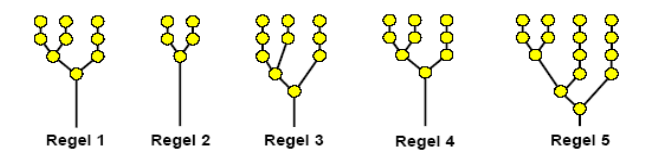
\includegraphics[width=0.8\textwidth]{figures/kap7/rule-mesh.png}
    \caption{Beispiel eines Regelnetzes}
    \label{fig:xps-rule-mesh}
\end{figure}

\begin{figure}[H]
    \centering
    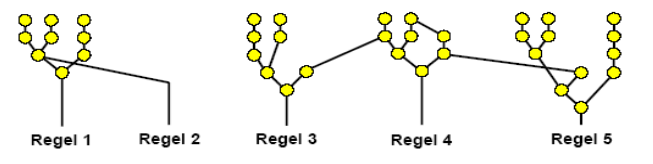
\includegraphics[width=0.8\textwidth]{figures/kap7/combined-rule-mesh.png}
    \caption{Kombinierte Regelnetze}
    \label{fig:xps-rule-mesh-combined}
\end{figure}

\section{Konfliktaufl�sung von Regelsystemen}

In vielen F�llen sind mehrere Regeln anwendbar, so dass sich die Frage stellt, welche Regeln man anwenden sollte. Die Antwort auf diese Frage h�ngt von der Reihenfolge der Regeln in der Regelbasis ab. In kommutativen Systemen kann eine schlechte Wahl der Regeln zu langen L�sungen f�hren. In nicht-kommutativen Systemen kann die Schwierigkeit der Suche aufgrund der R�ckverfolgung exponentiell sein. 

\paragraph{Ansatz 1: Heuristische Regelauswahl}

Wie bei den meisten Suchproblemen k�nnen Heuristiken den Prozess effizienter machen. Ein g�ngiger Ansatz besteht darin, sich an der H�ufigkeit der verwendeten Regel zu orientieren, d. h. jede Regel darf nur einmal verwendet werden. Ansonsten kann es von Vorteil sein, Regeln zu bevorzugen, die auf den neuesten generierten Daten beruhen. Schlie�lich ist es auch m�glich, eine Implementierung zu erstellen, die auf spezifischen Merkmalen des Problems basiert. Das bedeutet, dass Regeln, die mehr mit dem aktuellen Problem zu tun haben, bevorzugt werden.

\paragraph{Ansatz 2: Meta-Regeln}

Metaregeln sind Regeln �ber Regeln. In diesem Fall w�re ein Ansatz, Regeln �ber die Auswahl von Regeln in Form von Regeln zu bilden. Einige Meta-Regeln w�ren zum Beispiel: Regeln mit billigeren Verfahren gegen�ber teuren Verfahren bevorzugen, Regeln mit weniger gef�hrlichen Ans�tzen gegen�ber gef�hrlicheren Ans�tzen bevorzugen, Regeln von Experten gegen�ber Anf�ngern bevorzugen.

\section{Aufgaben bei der Entwicklung eines Expertensystems}

Um ein Expertensystem zu entwickeln, m�ssen bestimmte Schritte unternommen werden. An erster Stelle steht die Durchf�hrung einer Machbarkeitsanalyse. Expertensysteme sind nur in bestimmten Problemf�llen anwendbar, daher ist es wichtig, sich zu vergewissern, dass ein Expertensystem der richtige Methode ist. 

Danach ist es wichtig zu entscheiden, wie mit dem System interagiert werden soll. Das bedeutet, dass festgelegt werden muss, welche Aufgaben unterst�tzt werden sollen und welche Art von Dialog zwischen Benutzern und Experten gef�hrt werden muss.

Sobald dies erreicht ist, ist der n�chste Schritt der Wissenserwerb. Es m�ssen Experten gefunden und ihr Wissen gesammelt werden. Hier ist es wichtig, die richtigen Fragen zu stellen, um das gegebene Problem zu l�sen.

Als N�chstes folgt die Umsetzung des Wissens in Regeln, die Implementierung der Regeln in ein wissensbasiertes System und dann das Testen.